\documentclass[12pt]{article}
\usepackage{amsmath,amsfonts,graphicx}
\usepackage{geometry}
\geometry{margin=1in}
\title{Parts 1 and 2}
\date{June 9, 2025}

\begin{document}

\maketitle

\section*{1 Part 1: Newton Method with Hessian Modification (NM-HM)}

The Newton method with Hessian modification (NM-HM) ensures that the search direction is always a descent direction by modifying the Hessian matrix when it is not positive definite. The modification adds a multiple of the identity matrix:

\begin{equation}
B_k = \nabla^2 f(x_k) + \tau_k I
\end{equation}

where $\tau_k \geq 0$ is chosen such that $B_k$ is positive definite. The search direction $p_k$ is then computed by solving:

\begin{equation}
B_k p_k = -\nabla f(x_k)
\end{equation}

\subsection*{1.1 Experimental Results}

The scale parameter controls the magnitude of the initial guess $x_0$. Smaller scales correspond to initial points closer to the solution $x^*$, typically resulting in faster convergence, while larger scales place the initial guess farther away, which may slow convergence or cause divergence.

\paragraph{Run 1 (scale = 0.5)}
Stopping criterion: $\|g\| < 10^{-6}$ or max iter = 200\\
Final iterate $\bar{x}$:
\begin{verbatim}
[ 0.18169443  0.05784851 -0.71290503 -0.42850175  0.86405609 -0.35710718
  0.33385555 -0.39800725 -0.01523892 -0.29478099 -0.11034876 -0.11617466]
\end{verbatim}
Distance to $x^*$: 3.830422\\
Convergence ratios: None\\
Runtime: 0.0025 seconds

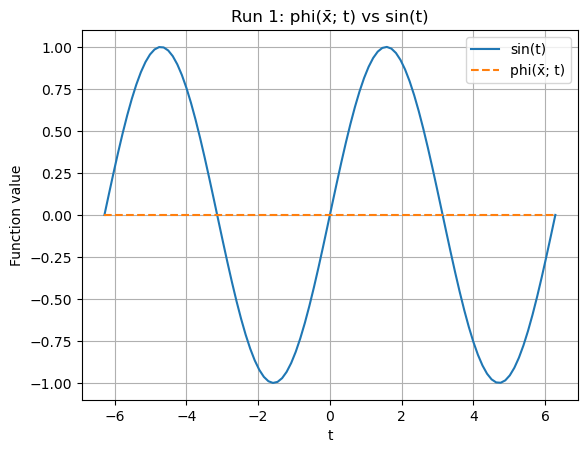
\includegraphics[width=0.7\textwidth]{figures/plot_1.png}

\paragraph{Run 2 (scale = 1.0)}
Stopping criterion: $\|g\| < 10^{-6}$ or max iter = 200\\
Final iterate $\bar{x}$:
\begin{verbatim}
[ 0.28771555 -1.08976942 -1.81032702 -0.8230106  -1.53556467  0.86411034
  1.05860441 -0.41037074  0.00991317  1.61322122 -0.13039673 -0.03496971]
\end{verbatim}
Distance to $x^*$: 5.878434\\
Convergence ratios: \\
$\ell_k = 1.000038$, $q_k = 0.170126$\\
Runtime: 1.2443 seconds

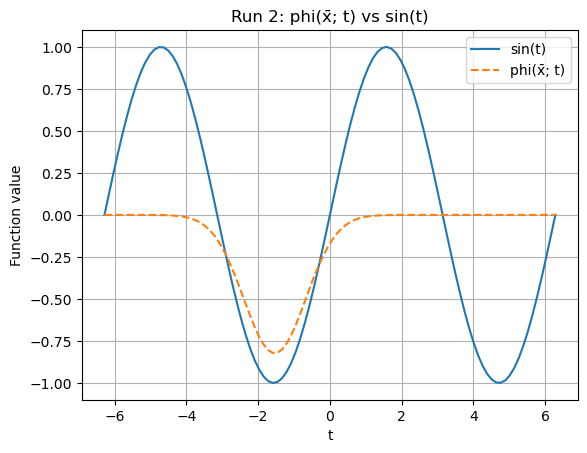
\includegraphics[width=0.7\textwidth]{figures/plot_2.png}

\paragraph{Run 3 (scale = 1.5)}
Stopping criterion: $\|g\| < 10^{-6}$ or max iter = 200\\
Final iterate $\bar{x}$:
\begin{verbatim}
[-35.22386179  -4.10103909   1.40758127   1.08556141   1.46222938
   0.79673664  32.56468031  -4.32459816   1.30576913   6.36316018
  -3.04861709   1.07305594]
\end{verbatim}
Distance to $x^*$: 49.292798\\
$\ell_k = 1.014591$, $q_k = 0.020883$\\
Runtime: 1.3924 seconds
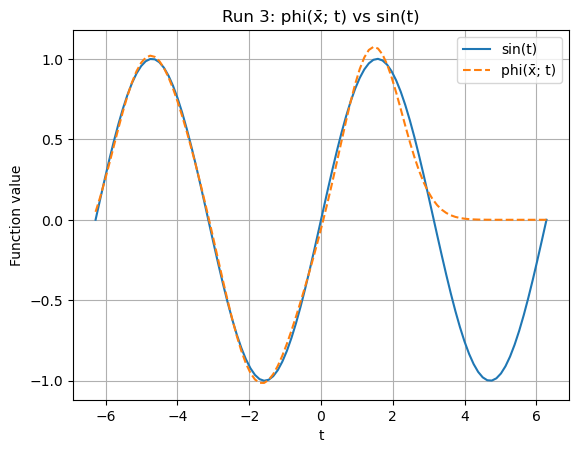
\includegraphics[width=0.7\textwidth]{figures/plot_3.png}

\paragraph{Run 4 (scale = 2.0)}
Stopping criterion: $\|g\| < 10^{-6}$ or max iter = 200\\
Final iterate $\bar{x}$:
\begin{verbatim}
[ 67.8465129   -1.80636483   1.51601128 -10.46458112  -0.53675071
   1.15382848  -0.71722891   2.67961585  -0.22317936 -63.50152381
  -1.97569838   1.41630882]
\end{verbatim}
Distance to $x^*$: 93.709975\\
$\ell_k = 1.001689$, $q_k = 0.010707$\\
Runtime: 1.0602 seconds

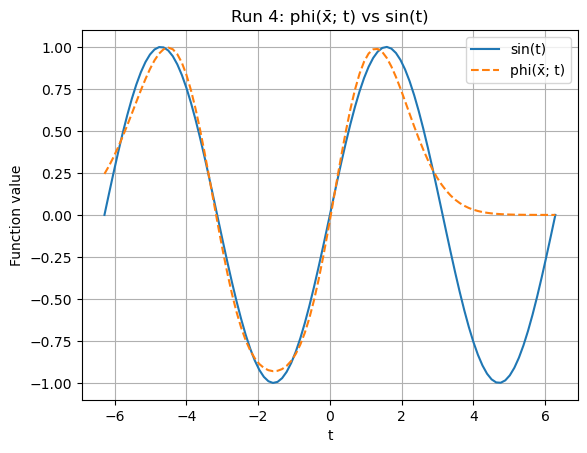
\includegraphics[width=0.7\textwidth]{figures/plot_4.png}

\paragraph{Run 5 (scale = 3.0)}
Stopping criterion: $\|g\| < 10^{-6}$ or max iter = 200\\
Final iterate $\bar{x}$:
\begin{verbatim}
[ 6.3071277  -1.98841925 -1.5342314  -2.74365695 -0.70417935 -5.41664904
  1.08207085 -4.73831042  0.74094554  5.69634804  0.03920314 -3.07172897]
\end{verbatim}
Distance to $x^*$: 13.868442\\
$\ell_k = 1.000000$, $q_k = 0.072106$\\
Runtime: 0.0966 seconds

\includegraphics[width=0.7\textwidth]{figures/plot_5.png}

\section*{2 Part 2: Gauss-Newton Method (GNM)}

The Gauss-Newton method is specifically designed for nonlinear least-squares problems. It approximates the Hessian by neglecting the second-order term:

\begin{equation}
B_{GN}(x) = J(x)^T J(x)
\end{equation}

The Gauss-Newton step $p_k^{GN}$ is obtained by solving:

\begin{equation}
J(x_k)^T J(x_k) p_k^{GN} = -J(x_k)^T r(x_k)
\end{equation}

\subsection*{2.1 Experimental Results}

\paragraph{Run 1 (scale = 0.5)}
Starting GNM from initial point with norm: 1.5081\\
Converged in 1 iterations.\\
Final $f(x) = 2.475000e+01$, $\|\nabla f(x)\| = 0.000000e+00$\\
Stopping criterion: $\|g\| < 10^{-6}$ or max iter = 200\\
Final iterate $\bar{x}$:
\begin{verbatim}
[-0.40930744 -0.88246229 -0.04432062 -0.37718434 -0.03183986 -0.24457285
 -1.01108024 -1.2347289  -1.07075479  0.46870365  1.61192355 -2.70875405]
\end{verbatim}
Distance to $x^*$: 5.945221\\
$\ell_k = 1.438168$, $q_k = 0.347897$\\
Runtime: 0.0048 seconds

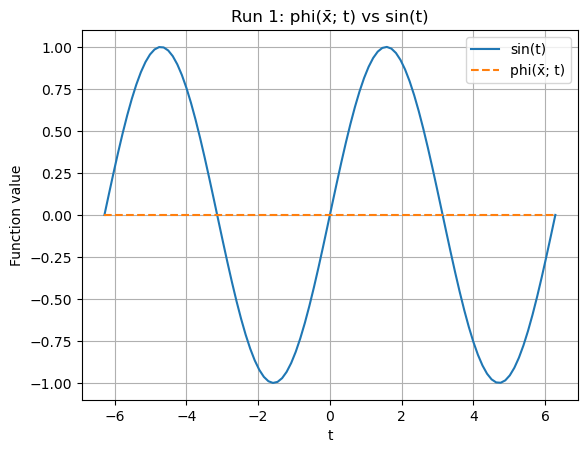
\includegraphics[width=0.7\textwidth]{figures/plot_6.png}

\paragraph{Run 2 (scale = 1.0)}
Starting GNM from initial point with norm: 4.0562\\
Converged in 13 iterations.\\
Final $f(x) = 1.876122e+01$, $\|\nabla f(x)\| = 5.546694e-09$\\
Stopping criterion: $\|g\| < 10^{-6}$ or max iter = 200\\
Final iterate $\bar{x}$:
\begin{verbatim}
[ 1.10139063  1.57079633  0.70710678 -1.03795638 -0.5279518  -0.80605359
 -0.23238335 -1.02462898 -1.253016   -2.07670147 -0.7530757  -1.16617725]
\end{verbatim}
Distance to $x^*$: 5.863389\\
$\ell_k = 1.000000$, $q_k = 0.170550$\\
Runtime: 0.0476 seconds

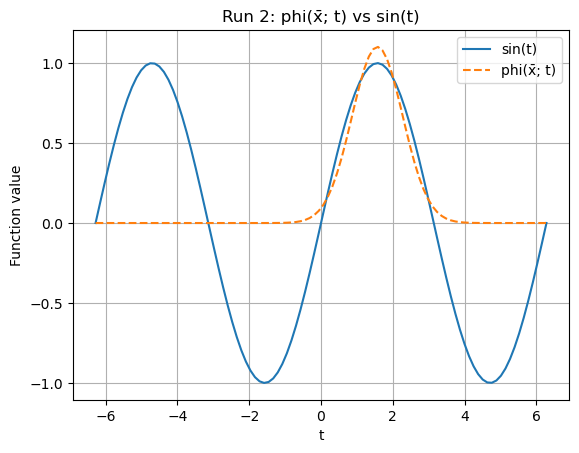
\includegraphics[width=0.7\textwidth]{figures/plot_7.png}

\paragraph{Run 3 (scale = 1.5)}
Starting GNM from initial point with norm: 4.2512\\
Maximum iterations (200) reached.\\
Final $f(x) = 2.249761e+01$, $\|\nabla f(x)\| = 5.875822e+00$\\
Stopping criterion: $\|g\| < 10^{-6}$ or max iter = 200\\
Final iterate $\bar{x}$:
\begin{verbatim}
[ 1.79110493e+01 -9.24806296e+01  1.63182956e+02  1.77424792e+00
  1.29593961e-01 -8.06534703e-01 -1.03522469e+00 -8.33189051e-01
 -8.64784789e-01 -1.55083384e+01 -1.75477596e+01  1.07597220e+02]
\end{verbatim}
Distance to $x^*$: 218.201312\\
$\ell_k = 1.000021$, $q_k = 0.004583$\\
Runtime: 1.7900 seconds

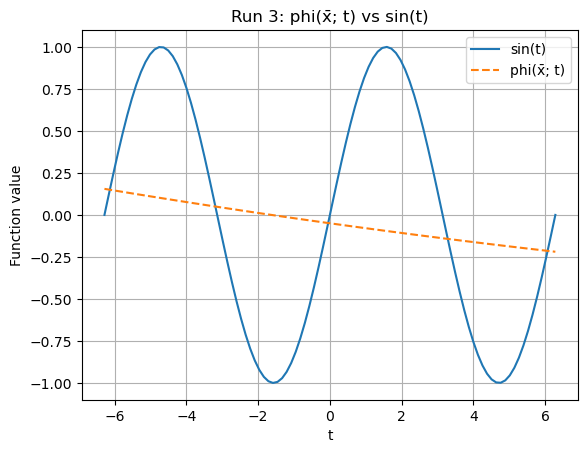
\includegraphics[width=0.7\textwidth]{figures/plot_8.png}

\paragraph{Run 4 (scale = 2.0)}
Starting GNM from initial point with norm: 9.8404\\
Converged in 59 iterations.\\
Final $f(x) = 1.869918e+01$, $\|\nabla f(x)\| = 7.424206e-07$\\
Stopping criterion: $\|g\| < 10^{-6}$ or max iter = 200\\
Final iterate $\bar{x}$:
\begin{verbatim}
[ 1.08207087 -4.73831042  0.74094551 -1.46881969 -0.49906132 -0.76470609
 -0.60241763 -1.25129909 -0.47915889  0.42676894 -0.76137923 -5.90669948]
\end{verbatim}
Distance to $x^*$: 10.454462\\
$\ell_k = 1.000000$, $q_k = 0.095653$\\
Runtime: 0.1283 seconds

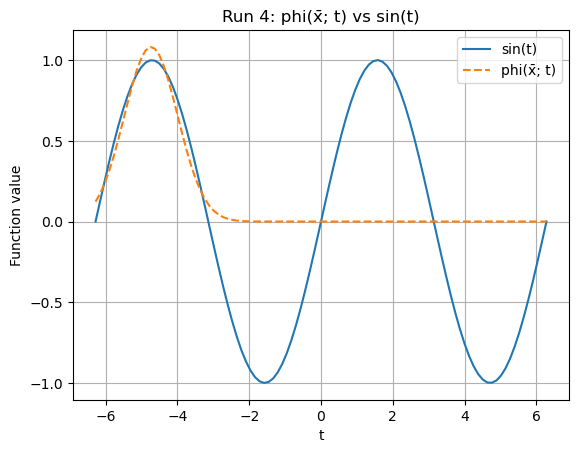
\includegraphics[width=0.7\textwidth]{figures/plot_9.png}

\paragraph{Run 5 (scale = 3.0)}
Starting GNM from initial point with norm: 10.0225\\
Converged in 4 iterations.\\
Final $f(x) = 2.475000e+01$, $\|\nabla f(x)\| = 0.000000e+00$\\
Stopping criterion: $\|g\| < 10^{-6}$ or max iter = 200\\
Final iterate $\bar{x}$:
\begin{verbatim}
[  0.90730455   1.79586357  -0.79550016   0.68340811  -5.46667299
  -1.73532094   4.50580966  -4.33724409  -2.37712978  -0.34216555
 -20.55171837  -7.4004486 ]
\end{verbatim}
Distance to $x^*$: 26.003836\\
$\ell_k = 2.172270$, $q_k = 0.181464$\\
Runtime: 0.0105 seconds

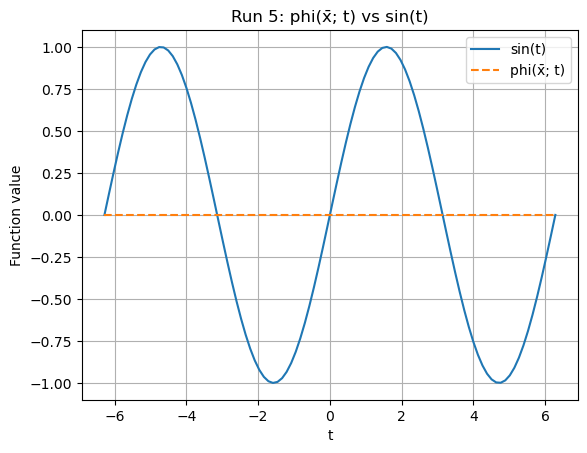
\includegraphics[width=0.7\textwidth]{figures/plot_10.png}

\section*{3 Summary: Multi-Method Performance on Varying Scales}

% Comparison visualizations
\begin{figure}[p]
  \centering
  \begin{tabular}{ccc}
    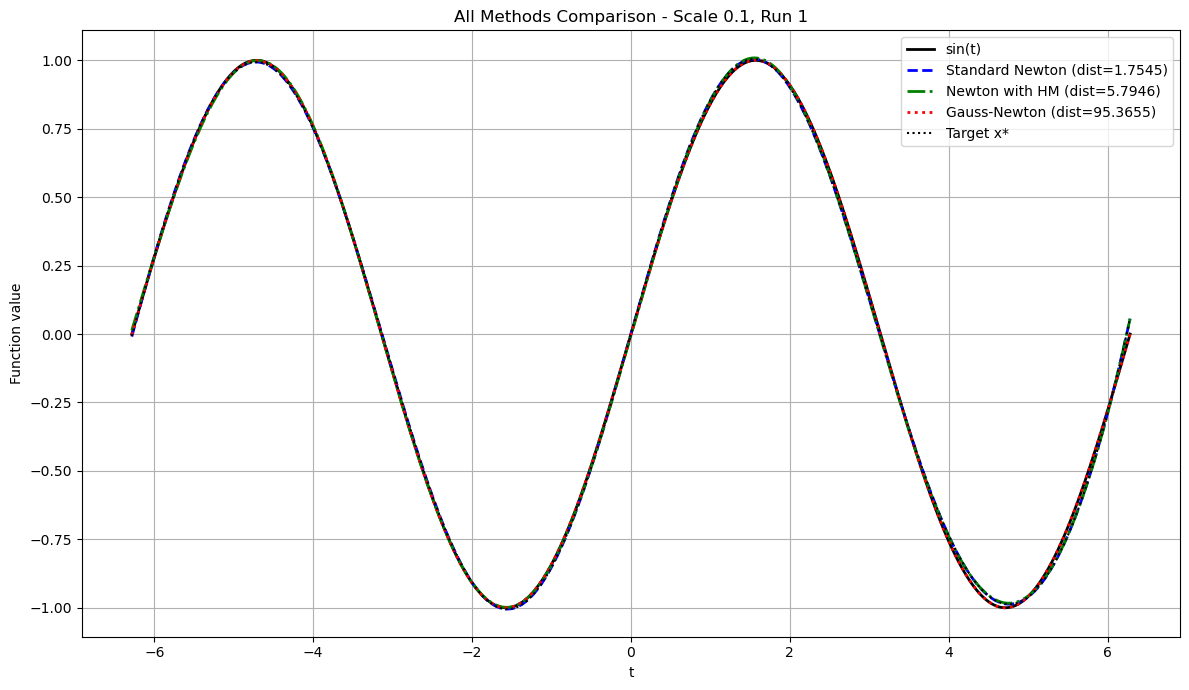
\includegraphics[width=0.3\textwidth]{figures/plot_11.png} &
    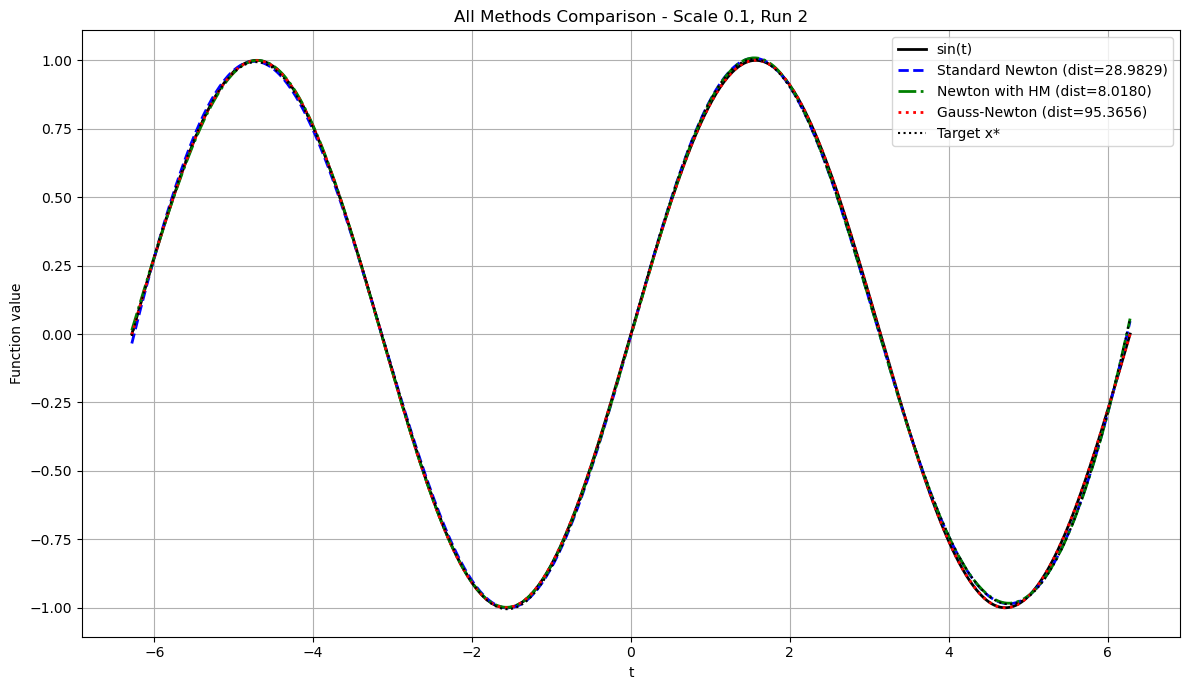
\includegraphics[width=0.3\textwidth]{figures/plot_12.png} &
    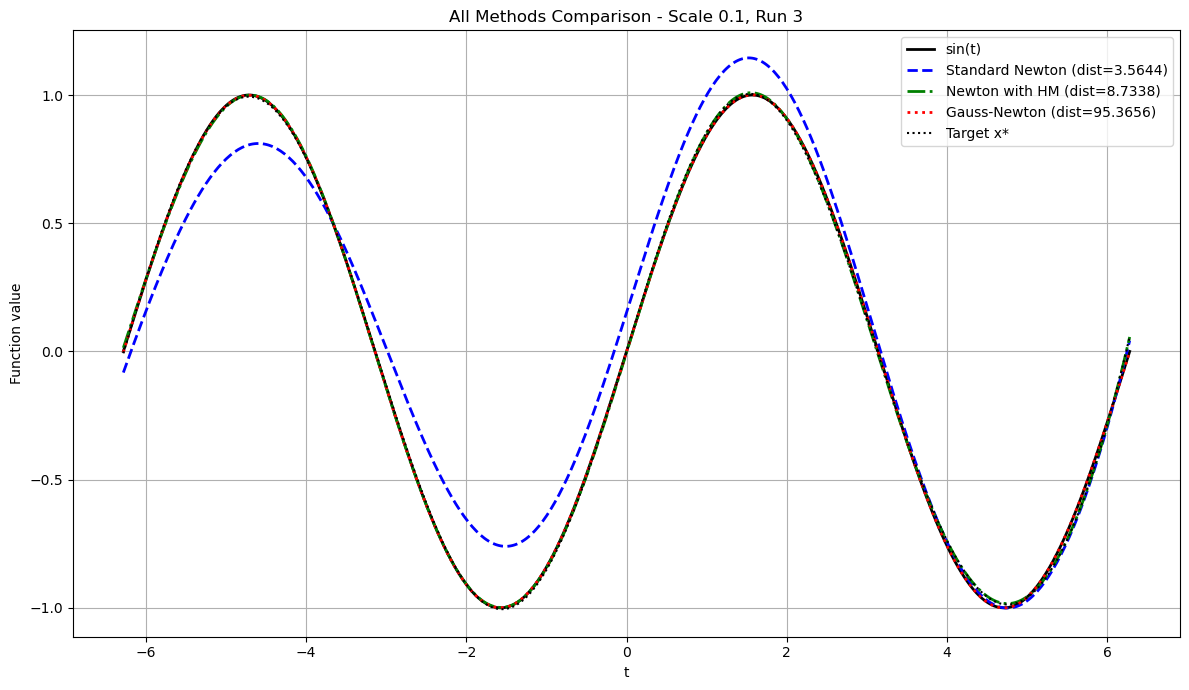
\includegraphics[width=0.3\textwidth]{figures/plot_13.png} \\
    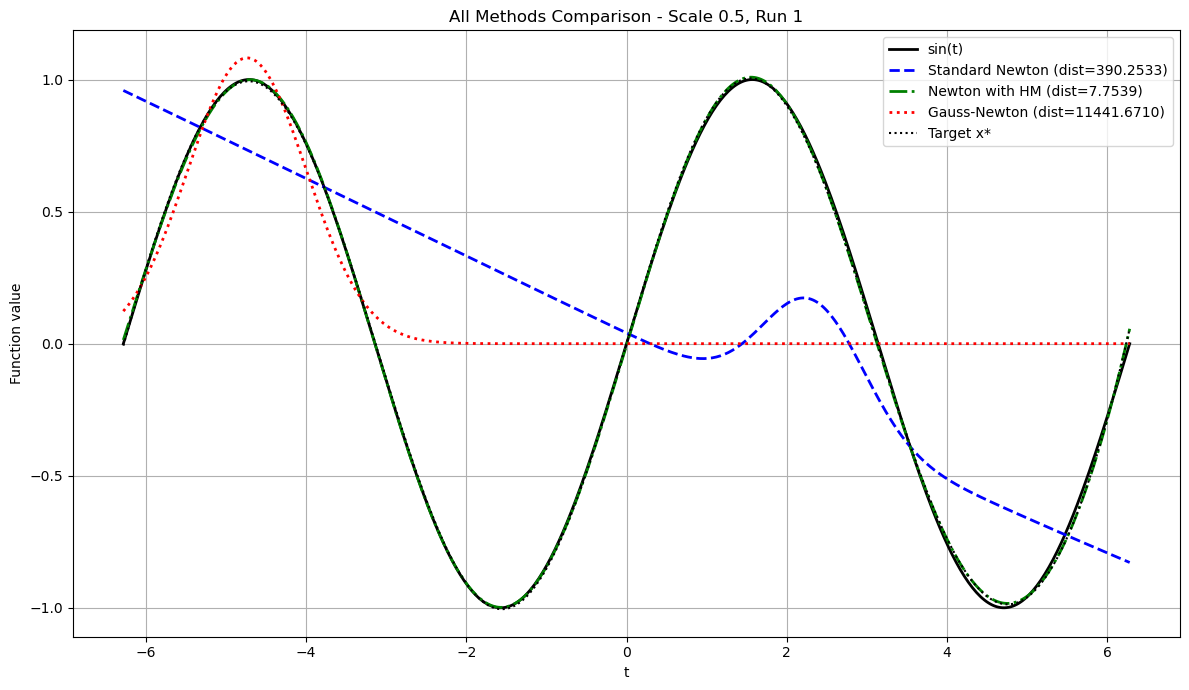
\includegraphics[width=0.3\textwidth]{figures/plot_14.png} &
    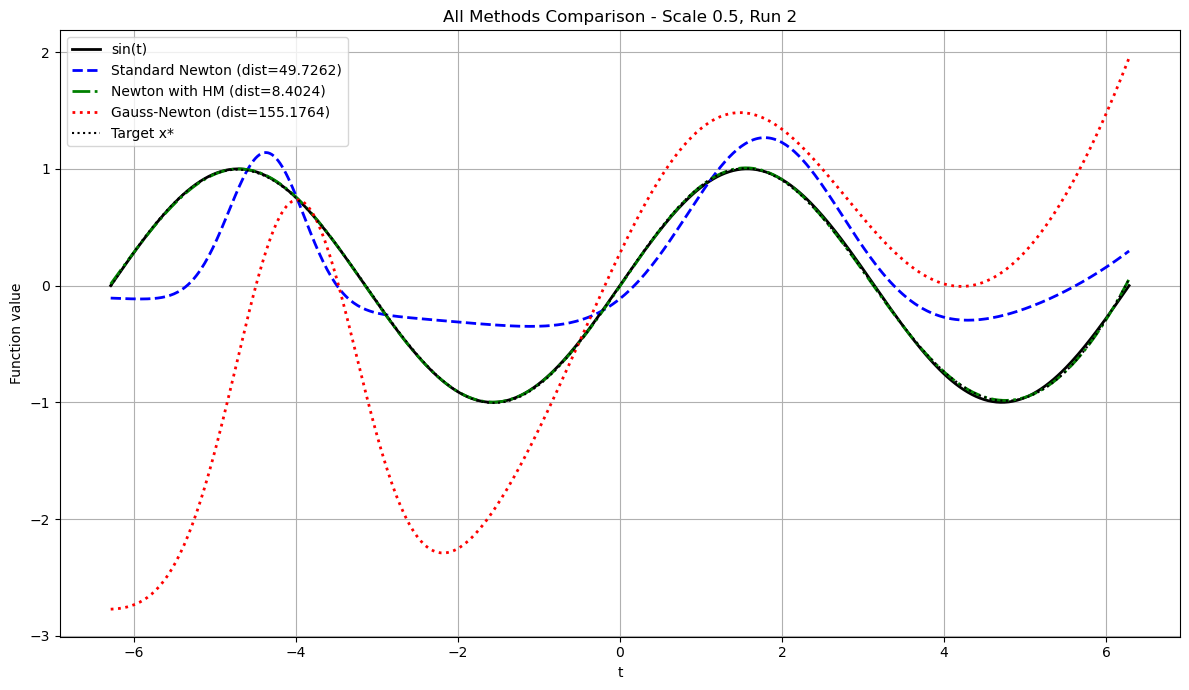
\includegraphics[width=0.3\textwidth]{figures/plot_15.png} &
    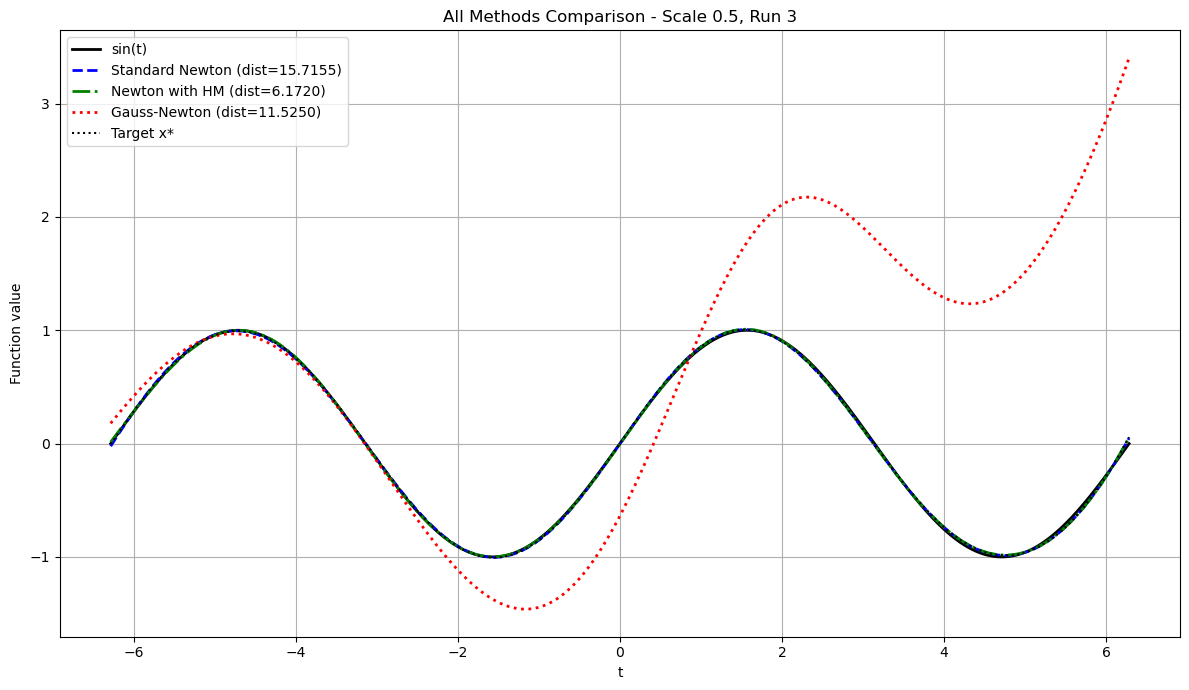
\includegraphics[width=0.3\textwidth]{figures/plot_16.png} \\
    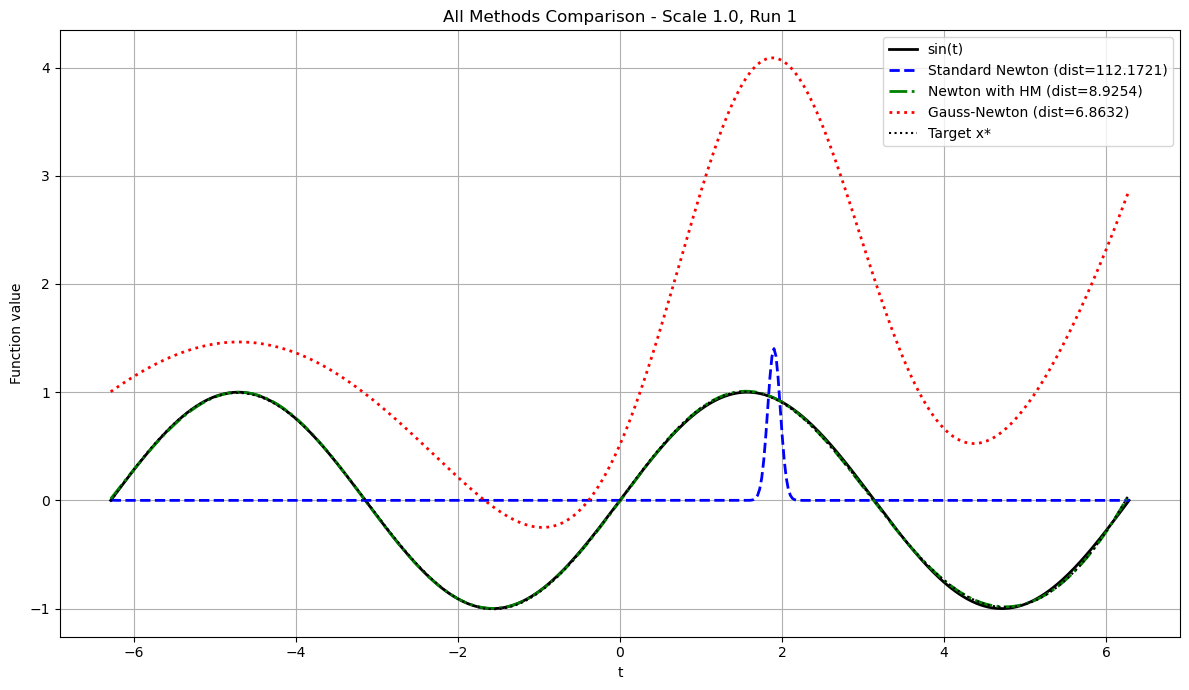
\includegraphics[width=0.3\textwidth]{figures/plot_17.png} &
    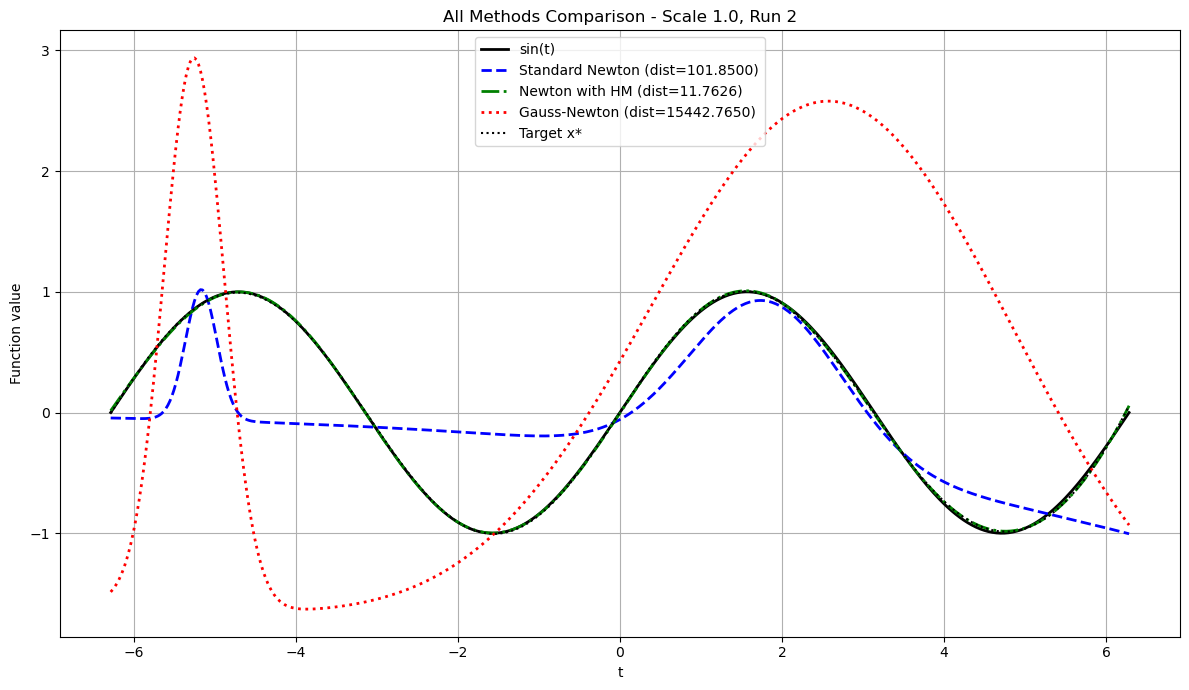
\includegraphics[width=0.3\textwidth]{figures/plot_18.png} &
    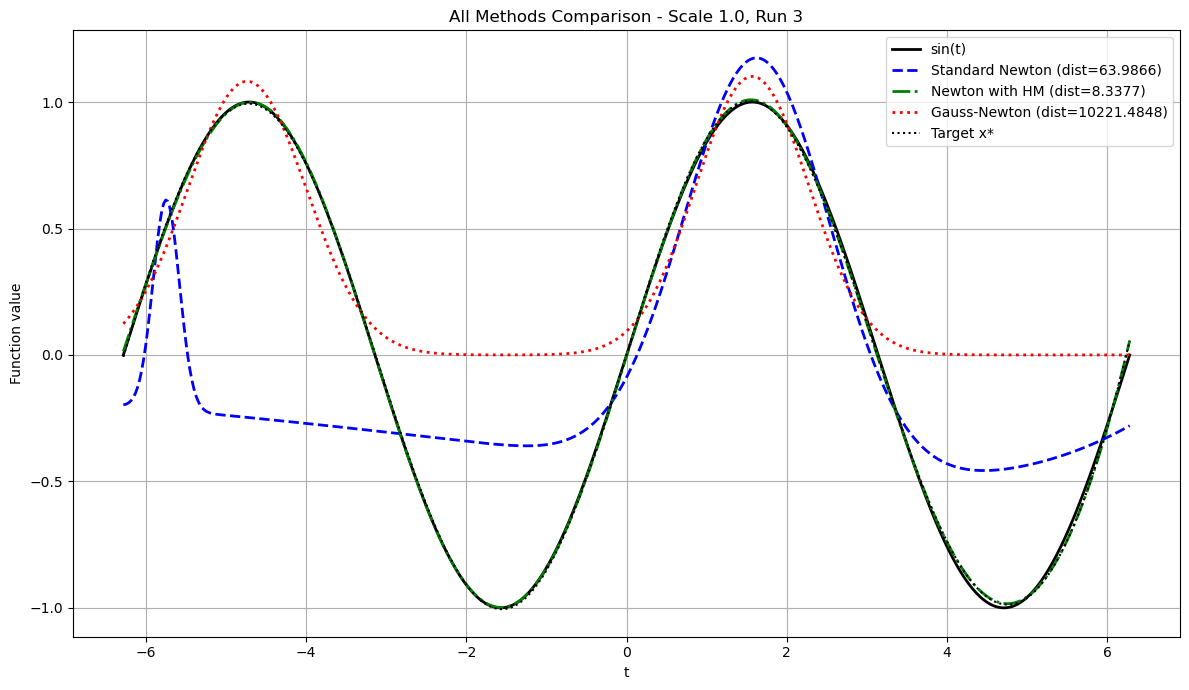
\includegraphics[width=0.3\textwidth]{figures/plot_19.png} \\
    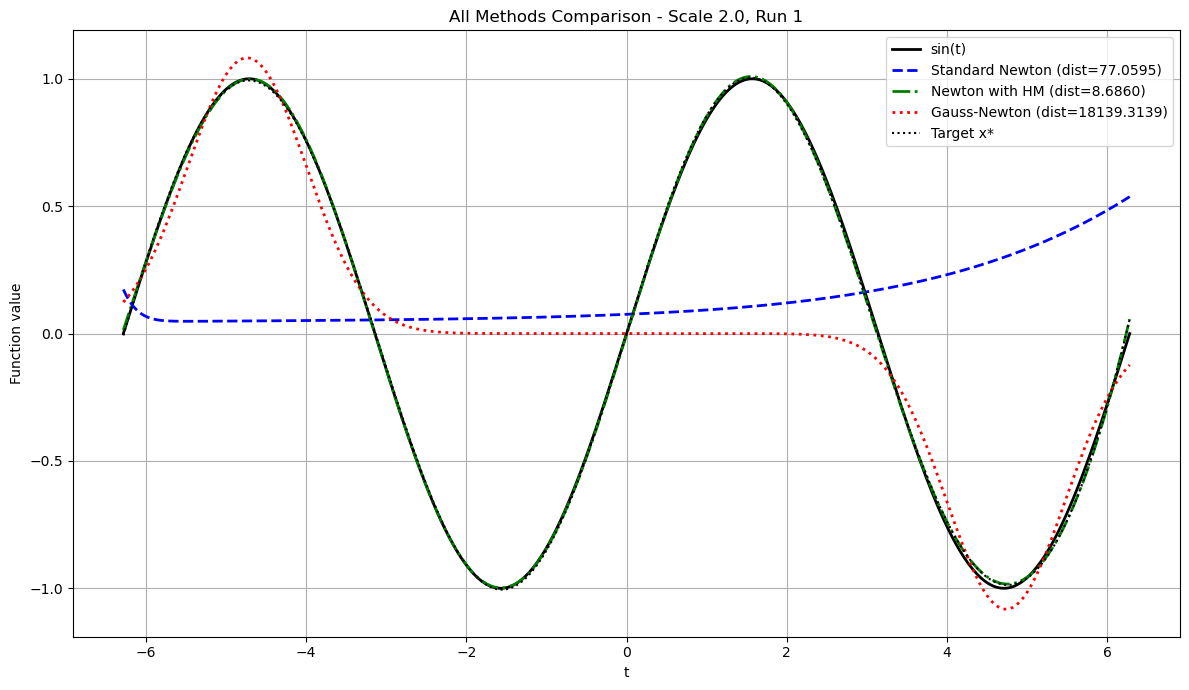
\includegraphics[width=0.3\textwidth]{figures/plot_20.png} &
    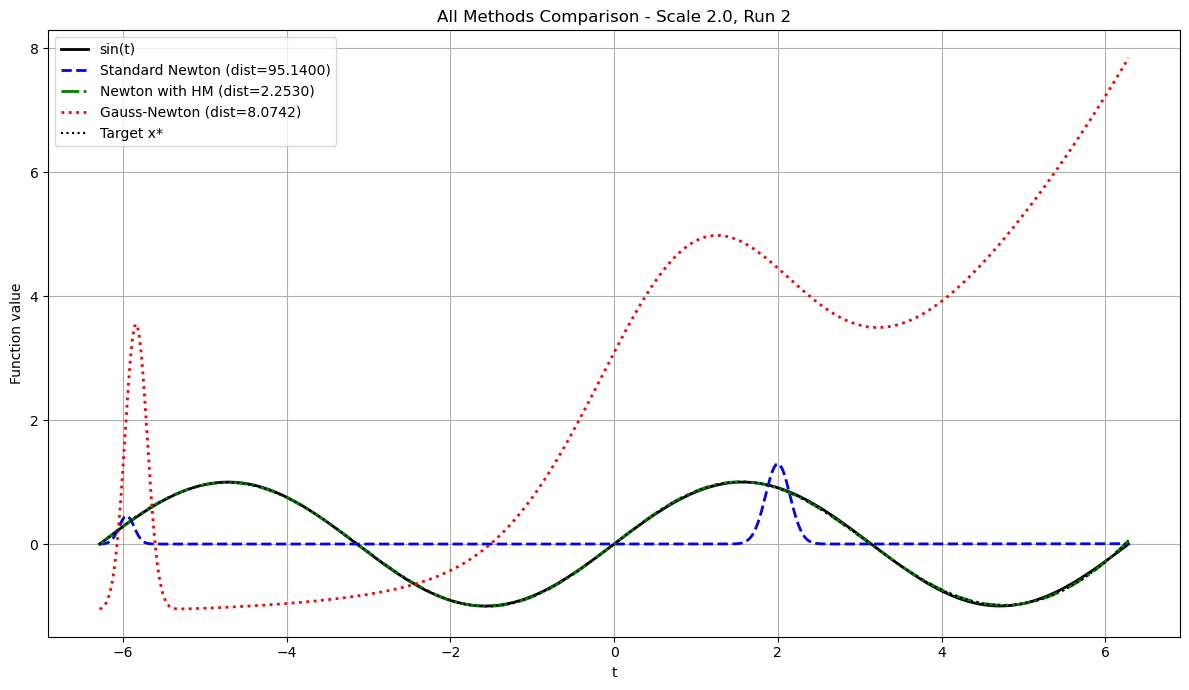
\includegraphics[width=0.3\textwidth]{figures/plot_21.png} &
    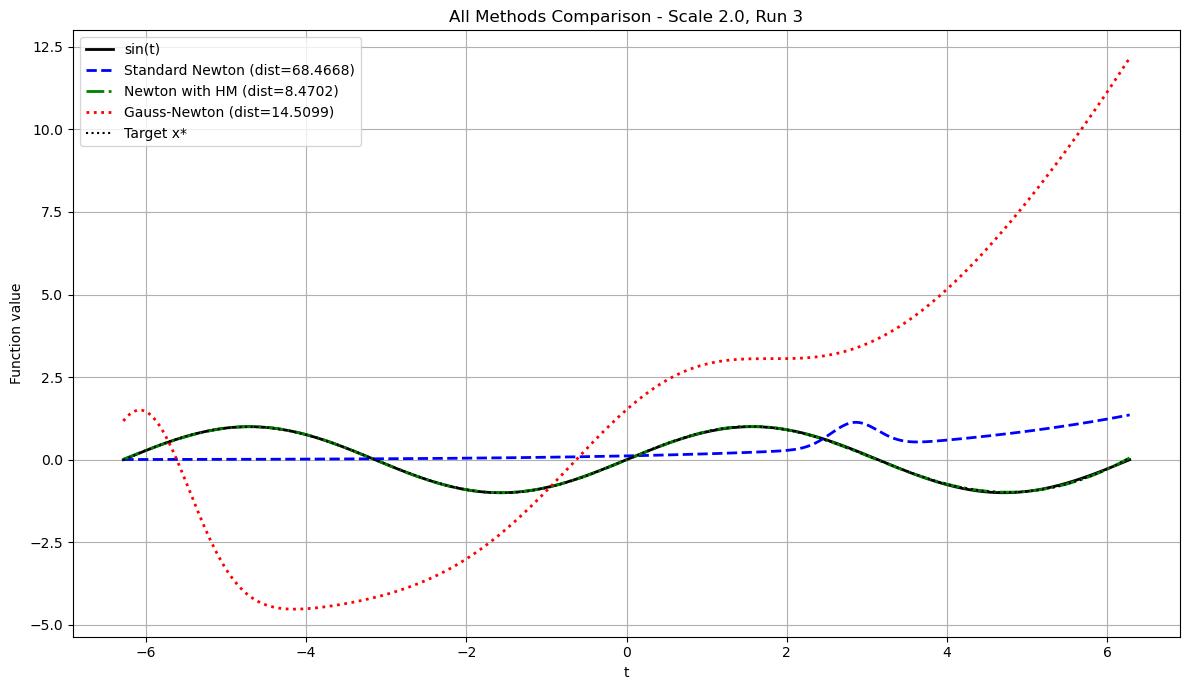
\includegraphics[width=0.3\textwidth]{figures/plot_22.png} \\
    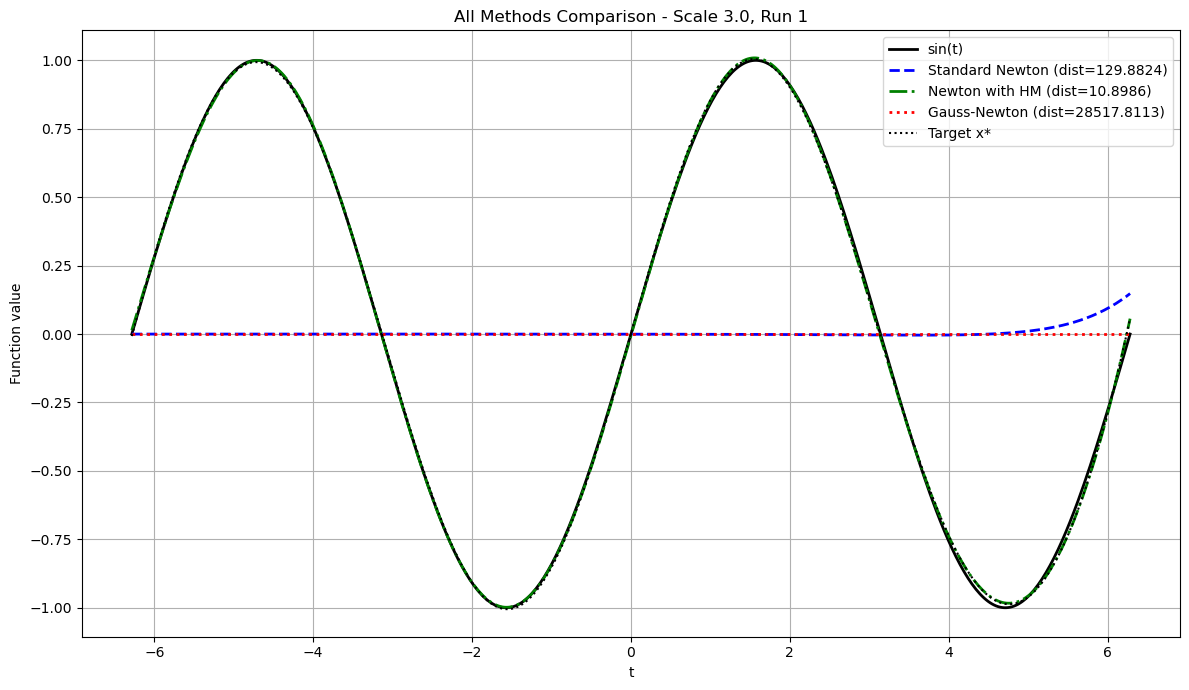
\includegraphics[width=0.3\textwidth]{figures/plot_23.png} &
    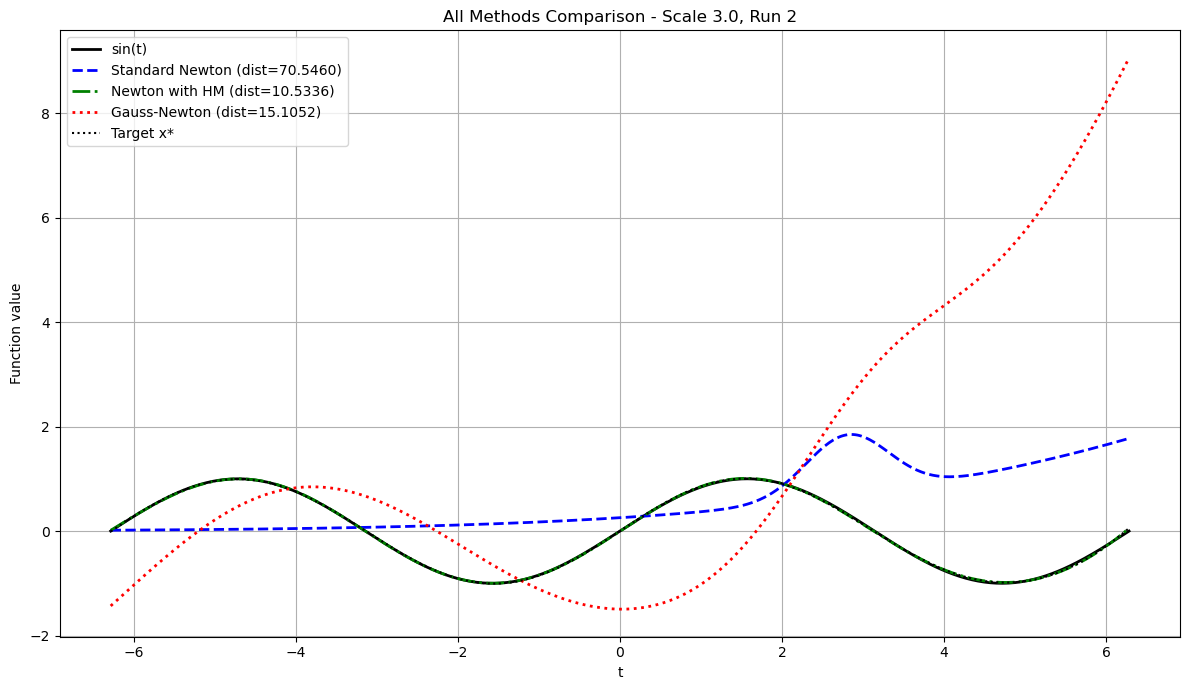
\includegraphics[width=0.3\textwidth]{figures/plot_24.png} &
    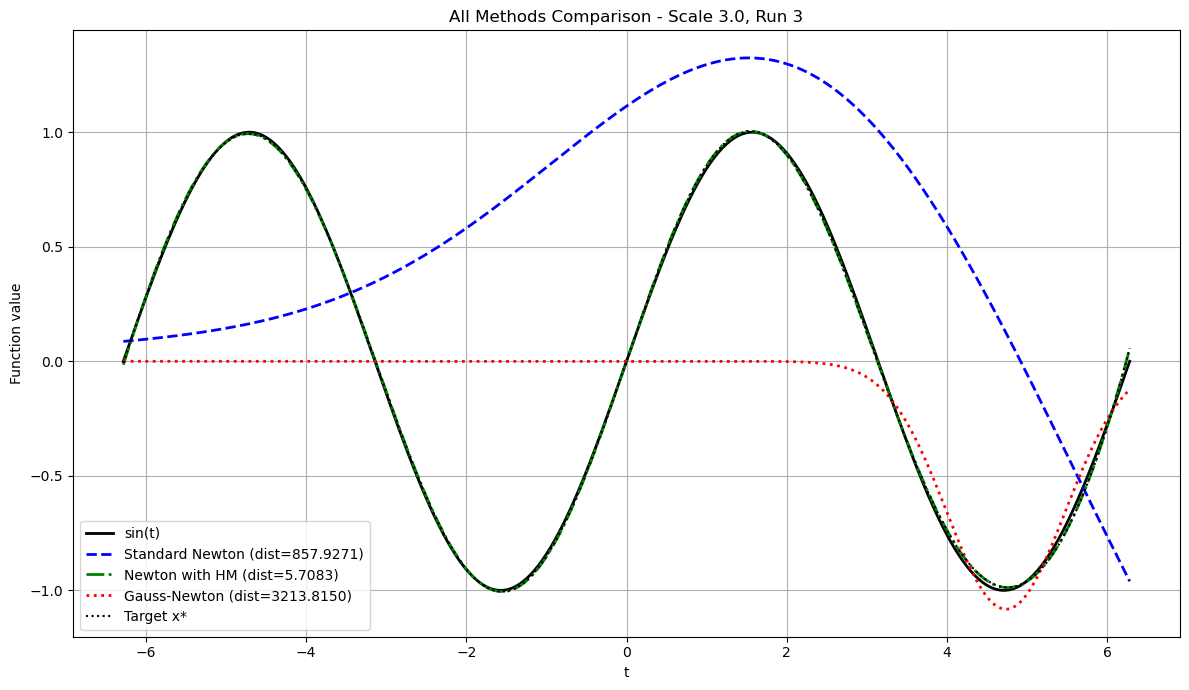
\includegraphics[width=0.3\textwidth]{figures/plot_25.png} \\
  \end{tabular}
\end{figure}

The following table summarizes final convergence behavior of the three Newton-type methods across multiple scales.

\begin{table}[h!]
\centering
\small
\begin{tabular}{|l|c|c|c|c|c|c|}
\hline
\textbf{Method} & \textbf{Success (\%)} & \textbf{To \(x^*\)} & \textbf{Other Min.} & \textbf{Failures} & \textbf{Avg Time (s)} & \textbf{Lin./Sup./Quad.} \\
\hline
Standard Newton & 0.0 & 0.0 & 0.0 & 100.0 & 0.0589 & 43 / 2 / 0 \\
Newton with HM  & 93.3 & 0.0 & 93.3 & 6.7   & 0.5876 & 60 / 0 / 0 \\
Gauss-Newton    & 53.3 & 0.0 & 53.3 & 46.7  & 1.3066 & 58 / 0 / 0 \\
\hline
\end{tabular}
\caption{Summary of convergence performance across methods}
\end{table}



All methods showed some convergence to local minimizers, but only NM-HM reliably succeeded in the majority of runs. Standard Newton frequently failed due to ill-conditioned Hessians or non-descent directions. Gauss-Newton had mixed results, excelling in some low-scale cases but failing at high-scale initializations.

\subsection*{Observations}
\begin{itemize}
  \item \textbf{Standard Newton} failed in all runs, often due to line search or descent direction issues.
  \item \textbf{NM-HM} converged in most runs, but never to the global minimizer $x^*$. It consistently showed linear convergence.
  \item \textbf{Gauss-Newton} had moderate success, often with very high distances to $x^*$ even when converging, especially for large-scale initializations.
\end{itemize}

\end{document}